\chapter{Grundlagen}

\section{Mathematische Grundlagen}

Diese Sektion beschreibt die wesentlichen mathematischen Konzepte, die in dieser Arbeit zur Verwendung kommen.

\subsection{Koordinatensysteme}

Ein wesentliches Konzept bei der Verarbeitung räumlicher Daten ist die Verwendung von Koordinatensystemen.
Sie werden genutzt um die Positionen von Daten und Objekten im Raum zu beschreiben.
Koordinatensysteme können für sich alleine stehen oder relativ zu anderen Koordinatensystemen.
Im Dreidimensionalen besitzt ein Koordinatensystem drei verschiedene Achsen (x, y und z-Achse), die jeweils im 90 Grad Winkel zueinander ausgerichtet sind.
Rotationen im Raum werden beschrieben als Rotationen um die jeweiligen Achsen.
Welche Achse in welche Richtung zeigt ist nicht eindeutig definiert.
Es gibt jedoch verschiedene Standards beziehungsweise Konventionen wie das links- oder rechtshändische Koordinatensystem.
In ROS wird konventionell ein rechtshändisches Koordinatensystem, abgebildet in Abbildung \ref{fig:ros_coordinate_sys} dargestellt. Dies wird im Folgenden ebenfalls als Standard verwendet.

\begin{figure}
		\centering
		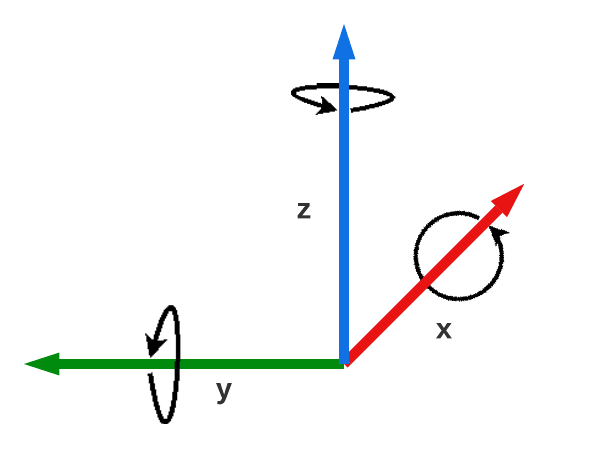
\includegraphics
			[scale=0.35]
			{ros_coordinate_sys}
		\caption
			[Caption for LOF]{Schematische Darstellung der Konvention für Koordinatensysteme im ROS Framework. Die z-Achse zeigt nach oben, die x-Achse nach vorne und die y-Achse nach links. Die Rotation um die Achsen ist entsprechend der Konvention im Uhrzeigersinn.}			                                                                                                                                     
		\label{fig:ros_coordinate_sys}
	\end{figure}

In der Robotik kommt es häufig vor, dass verschiedene (bewegliche) Komponenten relativ zu einem globalen Bezugssystem oder relativ zueinander beschrieben werden müssen. Die Bewegung eines übergeordneten Bezugssystems kann implizit für eine Veränderung der relativ zu diesem Bezugssystem platzierten Systeme führen.
Dies lässt sich anhand eines Arm-Roboters zeigen, der mehrere miteinander verbundene Gelenke hat. Bewegt sich ein Gelenk werden automatisch auch die am Arm weiter außen befindlichen Gelenke mitbewegt. Aus Sicht des bewegten, übergordneten Bezugssystems hat sich die Position der untergeordneten Gelenke nicht verändert, aus Sicht des globalen Bezugssystems, wie zum Beispiel dem Montierungspunkt des Roboters, allerdings schon.

In ROS werden Anhängigkeiten zwischen Bezugssystemen in einer Baumstruktur, genannt \textit{transformation tree (tf-tree)} dargestellt.
Die Wurzel dieser Baumstruktur ist das globale Bezugssystem, wie zum Beispiel der Ursprung einer globalen Karte oder der Startpunkt der Trajektorie eines Roboters.
Das globale Bezugssystem kann beliebig gewählt werden.
Auf diese Weise kann ein Koordinatensystem, welches relativ zu einem anderen gelegen ist im Baum als Kindknoten seinem Bezugssystem untergeordnet werden. Es wird nur die relative Transformation (s. Kapitel \ref{section:transformationen}) zwischen den Systemen im Baum gespeichert.
Dies hat den Vorteil, dass bei der Bewegung eines Systems die untergordneten Systeme nicht ebenfalls verändert werden müssen, da deren Transformationen relativ zum bewegten Bezugssystem angegeben sind und nicht global zur Wurzel des Baumes.
Abbildung \ref{fig:robot_tf} zeigt ein Beispiel für einen Roboter mit mehreren voneinander abhängigen System.


\begin{figure}
		\centering
		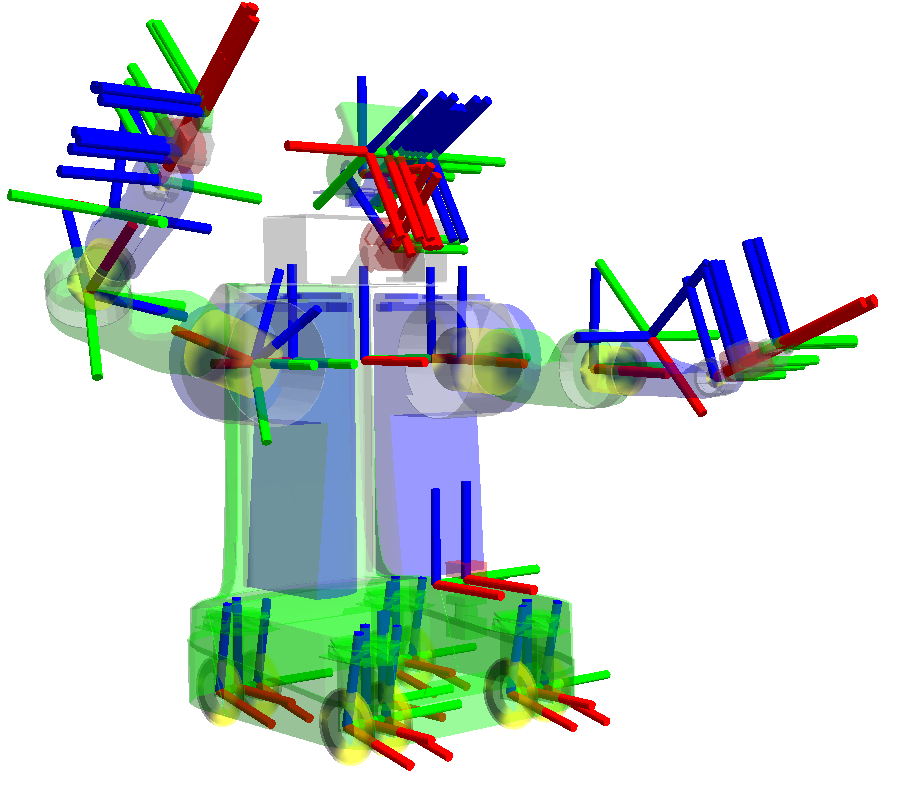
\includegraphics
			[scale=0.35]
			{robot_tf}
		\caption
			[Caption for LOF]{Schematische Darstellung eines Roboters und dessen beweglicher Teile. Die Ausrichtung der jeweiligen Gelenke wird mit einem lokalen Koordinatensystem beschrieben. Die globale Position einzelner Teile kann durch eine Verkettung der relativen Transformation in Richtung der Wurzel des Baumes bestimmt werden.
			Bild aus: TODO}			                                                                                                                                     
		\label{fig:robot_tf}
	\end{figure}

Auch räumliche Daten wie zum Beispiel Punktenwolken aus Laserscannern können relativ zu verschiedenen Koordinatensystemen gesehen werden.
So kann es nützlich sein die Punktwolke relativ zum Koordinatensystem des Scanners  

Räumliche Daten werden dabei immer relativ zu verschiedenen Koordinatensystemen gesehen.
Den Rahmen für diese relative, lokale Betrachtung von Daten liefert ein globales Koordinatensystem.
Das globale Koordinatensystem ist dabei im Folgenden immer das Koordinatensystem der Umgebungskarte.
Ein Beispiel für ein lokales Koordinatensystem ist die Position des aktuellen 

\subsubsection{Transformationen}
\label{section:transformationen}

TODO:

Schreiben über Transformationen
Erlären unterschiedlicher Repräsentationen.
KURZ auf Quaternions eingehen.
Transformationen zwischen Koordinatensystemen

\section{SLAM}

1. Grundlagen von SLAM beschreiben
-> Varianten des SLAM
-> Bezug zu HATSDF-SLAM
2. Vorraussetzungen (Repräsentationen für Posen (Pfad) und Umgebung)
3. Überleitungen in weitere Sektionen machen
	-> Loop Closure als mögliche Verbesserung des SLAM
	-> TSDF als Kartenrepräsentation
		-> auf Vorteile von TSDF eingehen (z.B. einfache Integration in Marching Cubes Algorithmus)


\section{Loop Closure}
\label{section:loop_closure_basics}

Warum wird Loop Closure benötigt?
Welchen Mehrwert gibt es?
Wie wäre ein grundlegendes vorgehen?
verweisen auf Loop-Closure Kapitel

\section{TSDF}